\documentclass{standalone}
\usepackage{tikz}
\usetikzlibrary{patterns, positioning}


\begin{document}
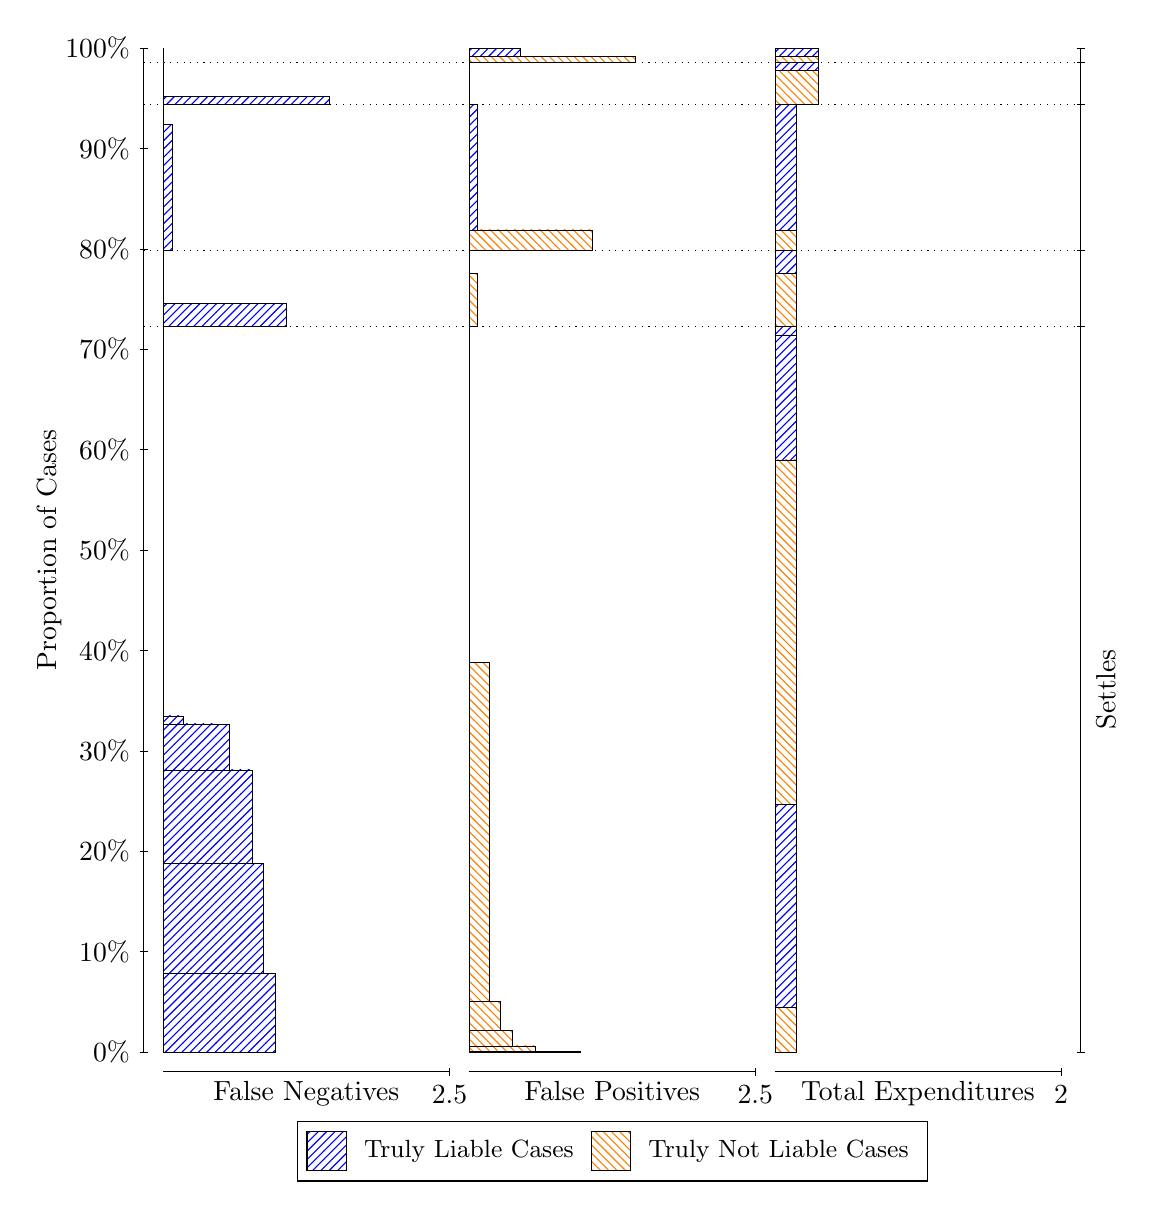
\begin{tikzpicture}
\draw[black, very thin] (1.5,1.75) -- (1.5,14.5);
\node[rotate=90, text=black, anchor=center] at (0.3, 8.125) {Proportion of Cases};
\draw[black, very thin] (1.45,1.75) -- (1.55,1.75);
\node[text=black, anchor=east] at (1.45, 1.75) {0\%};
\draw[black, very thin] (1.45,3.025) -- (1.55,3.025);
\node[text=black, anchor=east] at (1.45, 3.025) {10\%};
\draw[black, very thin] (1.45,4.3) -- (1.55,4.3);
\node[text=black, anchor=east] at (1.45, 4.3) {20\%};
\draw[black, very thin] (1.45,5.575) -- (1.55,5.575);
\node[text=black, anchor=east] at (1.45, 5.575) {30\%};
\draw[black, very thin] (1.45,6.85) -- (1.55,6.85);
\node[text=black, anchor=east] at (1.45, 6.85) {40\%};
\draw[black, very thin] (1.45,8.125) -- (1.55,8.125);
\node[text=black, anchor=east] at (1.45, 8.125) {50\%};
\draw[black, very thin] (1.45,9.4) -- (1.55,9.4);
\node[text=black, anchor=east] at (1.45, 9.4) {60\%};
\draw[black, very thin] (1.45,10.675) -- (1.55,10.675);
\node[text=black, anchor=east] at (1.45, 10.675) {70\%};
\draw[black, very thin] (1.45,11.95) -- (1.55,11.95);
\node[text=black, anchor=east] at (1.45, 11.95) {80\%};
\draw[black, very thin] (1.45,13.225) -- (1.55,13.225);
\node[text=black, anchor=east] at (1.45, 13.225) {90\%};
\draw[black, very thin] (1.45,14.5) -- (1.55,14.5);
\node[text=black, anchor=east] at (1.45, 14.5) {100\%};

\draw[black, very thin] (13.4,1.75) -- (13.4,14.5);
\draw[black, very thin] (13.35,1.75) -- (13.45,1.75);
\node[anchor=west] at (13.35, 1.75) {};
\draw[black, very thin] (13.35,10.963) -- (13.45,10.963);
\node[anchor=west] at (13.35, 10.963) {};
\draw[black, very thin] (13.35,11.934) -- (13.45,11.934);
\node[anchor=west] at (13.35, 11.934) {};
\draw[black, very thin] (13.35,13.782) -- (13.45,13.782);
\node[anchor=west] at (13.35, 13.782) {};
\draw[black, very thin] (13.35,14.317) -- (13.45,14.317);
\node[anchor=west] at (13.35, 14.317) {};
\draw[black, very thin] (13.35,14.5) -- (13.45,14.5);
\node[anchor=west] at (13.35, 14.5) {};

\draw[black, very thin, pattern color=blue, pattern=north east lines] (1.75,1.75) rectangle (3.167,2.7524);
\draw[black, very thin, pattern color=blue, pattern=north east lines] (1.75,2.7524) rectangle (3.0217,4.1489);
\draw[black, very thin, pattern color=blue, pattern=north east lines] (1.75,4.1489) rectangle (2.8763,5.3326);
\draw[black, very thin, pattern color=blue, pattern=north east lines] (1.75,5.3326) rectangle (2.5857,5.9095);
\draw[black, very thin, pattern color=blue, pattern=north east lines] (1.75,5.9095) rectangle (2.4403,5.918);
\draw[black, very thin, pattern color=blue, pattern=north east lines] (1.75,5.918) rectangle (2.0043,6.0186);
\draw[black, very thin, pattern color=orange, pattern=north west lines] (1.75,6.0186) rectangle (1.75,10.963);
\draw[black, very thin, pattern color=blue, pattern=north east lines] (1.75,10.963) rectangle (3.3123,11.261);
\draw[black, very thin, pattern color=orange, pattern=north west lines] (1.75,11.261) rectangle (1.75,11.934);
\draw[black, very thin, pattern color=blue, pattern=north east lines] (1.75,11.934) rectangle (1.859,13.526);
\draw[black, very thin, pattern color=orange, pattern=north west lines] (1.75,13.526) rectangle (1.75,13.782);
\draw[black, very thin, pattern color=blue, pattern=north east lines] (1.75,13.782) rectangle (3.8573,13.887);
\draw[black, very thin, pattern color=orange, pattern=north west lines] (1.75,13.887) rectangle (1.75,14.317);
\draw[black, very thin, pattern color=orange, pattern=north west lines] (1.75,14.317) rectangle (1.75,14.389);
\draw[black, very thin, pattern color=blue, pattern=north east lines] (1.75,14.389) rectangle (1.75,14.5);
\draw[black, very thin, pattern color=orange, pattern=north west lines] (5.6333,1.75) rectangle (7.0503,1.7559);
\draw[black, very thin, pattern color=orange, pattern=north west lines] (5.6333,1.7559) rectangle (6.6143,1.7564);
\draw[black, very thin, pattern color=orange, pattern=north west lines] (5.6333,1.7564) rectangle (6.469,1.826);
\draw[black, very thin, pattern color=orange, pattern=north west lines] (5.6333,1.826) rectangle (6.1783,2.0272);
\draw[black, very thin, pattern color=orange, pattern=north west lines] (5.6333,2.0272) rectangle (6.033,2.3919);
\draw[black, very thin, pattern color=orange, pattern=north west lines] (5.6333,2.3919) rectangle (5.8877,6.6945);
\draw[black, very thin, pattern color=blue, pattern=north east lines] (5.6333,6.6945) rectangle (5.6333,10.963);
\draw[black, very thin, pattern color=orange, pattern=north west lines] (5.6333,10.963) rectangle (5.7423,11.636);
\draw[black, very thin, pattern color=blue, pattern=north east lines] (5.6333,11.636) rectangle (5.6333,11.934);
\draw[black, very thin, pattern color=orange, pattern=north west lines] (5.6333,11.934) rectangle (7.1957,12.189);
\draw[black, very thin, pattern color=blue, pattern=north east lines] (5.6333,12.189) rectangle (5.7423,13.782);
\draw[black, very thin, pattern color=orange, pattern=north west lines] (5.6333,13.782) rectangle (5.6333,14.212);
\draw[black, very thin, pattern color=blue, pattern=north east lines] (5.6333,14.212) rectangle (5.6333,14.317);
\draw[black, very thin, pattern color=orange, pattern=north west lines] (5.6333,14.317) rectangle (7.7407,14.389);
\draw[black, very thin, pattern color=blue, pattern=north east lines] (5.6333,14.389) rectangle (6.2873,14.5);
\draw[black, very thin, pattern color=orange, pattern=north west lines] (9.5167,1.75) rectangle (9.7892,2.3158);
\draw[black, very thin, pattern color=blue, pattern=north east lines] (9.5167,2.3158) rectangle (9.7892,4.8961);
\draw[black, very thin, pattern color=orange, pattern=north west lines] (9.5167,4.8961) rectangle (9.7892,9.2683);
\draw[black, very thin, pattern color=blue, pattern=north east lines] (9.5167,9.2683) rectangle (9.7892,10.848);
\draw[black, very thin, pattern color=orange, pattern=north west lines] (9.5167,10.848) rectangle (9.7892,10.854);
\draw[black, very thin, pattern color=blue, pattern=north east lines] (9.5167,10.854) rectangle (9.7892,10.963);
\draw[black, very thin, pattern color=orange, pattern=north west lines] (9.5167,10.963) rectangle (9.7892,11.636);
\draw[black, very thin, pattern color=blue, pattern=north east lines] (9.5167,11.636) rectangle (9.7892,11.934);
\draw[black, very thin, pattern color=orange, pattern=north west lines] (9.5167,11.934) rectangle (9.7892,12.189);
\draw[black, very thin, pattern color=blue, pattern=north east lines] (9.5167,12.189) rectangle (9.7892,13.782);
\draw[black, very thin, pattern color=orange, pattern=north west lines] (9.5167,13.782) rectangle (10.062,14.212);
\draw[black, very thin, pattern color=blue, pattern=north east lines] (9.5167,14.212) rectangle (10.062,14.317);
\draw[black, very thin, pattern color=orange, pattern=north west lines] (9.5167,14.317) rectangle (10.062,14.389);
\draw[black, very thin, pattern color=blue, pattern=north east lines] (9.5167,14.389) rectangle (10.062,14.5);
\draw[black, dotted] (1.5,10.963) -- (13.4,10.963);
\draw[black, dotted] (1.5,11.934) -- (13.4,11.934);
\draw[black, dotted] (1.5,13.782) -- (13.4,13.782);
\draw[black, dotted] (1.5,14.317) -- (13.4,14.317);
\draw[black, very thin] (1.75,1.5) -- (5.3833,1.5);
\node[text=black, anchor=north] at (3.5667, 1.5) {False Negatives};
\draw[black, very thin] (5.3833,1.45) -- (5.3833,1.55);
\node[text=black, anchor=north] at (5.3833, 1.45) {2.5};

\draw[black, very thin] (5.6333,1.5) -- (9.2667,1.5);
\node[text=black, anchor=north] at (7.45, 1.5) {False Positives};
\draw[black, very thin] (9.2667,1.45) -- (9.2667,1.55);
\node[text=black, anchor=north] at (9.2667, 1.45) {2.5};

\draw[black, very thin] (9.5167,1.5) -- (13.15,1.5);
\node[text=black, anchor=north] at (11.333, 1.5) {Total Expenditures};
\draw[black, very thin] (13.15,1.45) -- (13.15,1.55);
\node[text=black, anchor=north] at (13.15, 1.45) {2};

\node[text=black, centered, rotate=90] at (13.72, 6.3566) {Settles};





\draw (7.449999999999999,1.5) node[draw=none] (baseCoordinate) {};
\begin{scope}[align=center]
        \matrix[scale=0.5, draw=black, below=0.5cm of baseCoordinate, nodes={draw}, column sep=0.1cm]{
            \node[rectangle, draw, minimum width=0.5cm, minimum height=0.5cm, pattern color=blue, pattern=north east lines] {}; &
            \node[draw=none, font=\small, text=black] (B) {Truly Liable Cases}; &
            \node[rectangle, draw, minimum width=0.5cm, minimum height=0.5cm, pattern color=orange, pattern=north west lines] {}; &
            \node[draw=none, font=\small, text=black] (B) {Truly Not Liable Cases}; \\
            };
\end{scope}

\end{tikzpicture}
\end{document}